\documentclass[12pt, a4paper]{article}

% --- Pacotes Básicos ---
\usepackage[utf8]{inputenc}
\usepackage[T1]{fontenc}
\usepackage[portuguese]{babel}
\usepackage{geometry}
\geometry{margin=2.5cm}
\usepackage{amsmath}
\usepackage{amsfonts}
\usepackage{hyperref}
\usepackage{booktabs}
\usepackage{listings}
\usepackage{xcolor}
\usepackage{tikz}

% --- Configuração de Cores e Código (Listings) ---
\definecolor{codegray}{rgb}{0.5,0.5,0.5}
\definecolor{backcolour}{rgb}{0.95,0.95,0.92}

\lstset{
    backgroundcolor=\color{backcolour},
    basicstyle=\ttfamily\small,
    breaklines=true,
    captionpos=b,
    keepspaces=true,
    numbers=left,
    numberstyle=\tiny\color{codegray},
    showspaces=false,
    showstringspaces=false,
    frame=single
}

% =========================================================================
% O DOCUMENTO COMEÇA AQUI
% =========================================================================
\begin{document}

% --- Capa do Relatório ---
\begin{titlepage}
    \centering
    \vspace*{1cm}
    
    % Instituição e Disciplina
    {\large \scshape Universidade do Minho} \\
    \vspace{0.2cm}
    {\large \textbf{Departamento de Informática}} \\
    \vspace{0.2cm}
    {\large UC: Processamento de Linguagens} \\
    
    \vspace{3.5cm}
    
    % Linha divisória superior
    \rule{\linewidth}{0.6mm} \\[0.4cm]
    % Título e Subtítulo
    {\huge \bfseries Relatório do Trabalho Prático} \\[0.3cm]
    {\Large \color{gray} Desenvolvimento de um Compilador de Fortran 77} \\[0.4cm]
    % Linha divisória inferior
    \rule{\linewidth}{0.6mm} \\
    
    \vfill
    
    % Secção de Autores organizada
    {\large \textbf{Autores:}} \\[0.3cm]
    \begin{tabular}{ll}
        A107336 & Alexandre Ferrete \\
        A106872 & Dinis Costa \\
        A107333 & Lucas Martins \\
    \end{tabular}
    
    \vfill
    
    % Data no fundo
    {\large 17 de Maio de 2026}
    
\end{titlepage}

\newpage
\tableofcontents

% --- Secção 1: Introdução ---
\newpage
\section{Introdução}
Este projeto consiste na implementação de raiz de um compilador de \textit{Fortran 77} no âmbito das temáticas estudadas em Processamento de Linguagens. O compilador foi inteiramente desenvolvido na linguagem \textit{Python}, utilizando ferramentas de suporte \textit{PLY}. O código máquina gerado pelo programa tem como alvo a Máquina Virtual disponibilizada pela equipa docente. O projeto conta ainda com a fase de valorizações, incluindo otimizações e definição e chamada de subprogramas.

% --- Secção 2: Opções de Implementação ---
\section{Opções de Implementação}

\subsection{Formato do Código Fonte}
O grupo optou por suportar o \textbf{formato livre (free-form)}, em detrimento do formato de colunas fixas do Fortran 77 original. Esta decisão simplifica a especificação do analisador léxico e aproxima o ambiente de desenvolvimento das práticas modernas de escrita em Fortran, mantendo total compatibilidade com os exemplos do enunciado.

Os comentários são aceites em duas vertentes: linhas completas iniciadas pelos caracteres \texttt{C}, \texttt{c} ou \texttt{*} (seguidos obrigatoriamente por um espaço), e comentários \textit{inline} delimitados pelo caractere \texttt{!}.

\subsection{Estrutura do Projeto}
\begin{lstlisting}[language=bash, caption=Estrutura de diretórios do projeto]
src/
    |-- __main__.py        # Ponto de entrada CLI do compilador
    |-- lexer.py           # Analise lexica (PLY lex)
    |-- parser.py          # Analise sintatica (PLY yacc)
    |-- ast_nodes.py       # Definicao dos nos da AST
    |-- semantic.py        # Analise semantica e verificacao de tipos
    |-- bm_codegen.py      # Gerador de codigo para a VM
    |-- optimizer.py       # Otimizacoes ao nivel do Bytecode (O1)
    |-- ast_optimizer      # Otimizacao de fluxo (O2)
    |-- builtin_defs.py    # Suporte a funcoes intrinsicas de Fortran

tests/
    |-- hello.f
    |-- fatorial.f
    |-- ...
\end{lstlisting}

\subsection{Análise Léxica (\texttt{lexer.py})}
O analisador léxico é responsável por processar o fluxo de texto bruto do ficheiro de origem e decompô-lo numa sequência ordenada de \textit{tokens}, descartando os elementos não necessários (espaços em branco e comentários). Utilizando o \texttt{ply.lex}, mapearam-se as palavras-chave da linguagem e os operadores fundamentais:

\begin{table}[h!]
\centering
\begin{tabular}{@{}lp{10cm}@{}}
\toprule
\textbf{Categoria} & \textbf{Exemplos} \\ \midrule
Palavras-chave & \texttt{PROGRAM, END, INTEGER, REAL, LOGICAL, IF, THEN, ELSE, DO, GOTO, CONTINUE, PRINT, READ, FUNCTION, SUBROUTINE, RETURN, CALL, ENDIF} \\
Ops. Aritméticos & \texttt{+, -, *, /, **} \\
Ops. Relacionais & \texttt{.EQ., .NE., .LT., .LE., .GT., .GE.} \\
Ops. Lógicos & \texttt{.AND., .OR., .NOT.} \\
Literais Lógicos & \texttt{.TRUE., .FALSE.} \\
Identificadores & \texttt{[a-zA-Z\_][a-zA-Z0-9\_]*} \\ \bottomrule
\end{tabular}
\end{table}

A nível de precedência léxica, os operadores compostos como a potência (\texttt{**}) foram especificados em funções dedicadas no PLY para garantir a sua captura prioritária antes dos operadores simples como a multiplicação (\texttt{*}).

\subsection{Análise Sintática e Árvore de Sintaxe Abstrata (\texttt{parser.py} e \texttt{ast\_nodes.py})}
O \textit{parser} valida se a sequência ordenada de \textit{tokens} respeita a estrutura gramatical definida para este subconjunto de Fortran 77. Recorrendo ao \texttt{ply.yacc}, foi construído um analisador do tipo LALR(1) que traduz o programa estruturado numa Árvore de Sintaxe Abstrata (AST). Os nós da árvore foram divididos logicamente em duas famílias base:
\begin{itemize}
    \item \textbf{Expressions:} Nós computacionais que processam e devolvem um tipo concreto de valor (ex: \texttt{BinOp}, \texttt{UnaryOp}, \texttt{Literal}).
    \item \textbf{Statements:} Nós imperativos que executam uma instrução ou alteram o fluxo de controlo do programa, sem produção de valor direto (ex: \texttt{Assignment}, \texttt{IfStmt}, \texttt{DoStmt}).
\end{itemize}


\subsection{Análise Semântica (\texttt{semantic.py})}

O analisador semântico realiza a validação lógica do programa antes da geração de código. Este módulo constrói e gere uma Tabela de Símbolos estruturada para validar os diferentes escopos do programa.

As principais tarefas executadas por este componente são:
\begin{itemize}
    \item \textbf{Validação de Declarações:} Garante que todas as variáveis foram declaradas antes de serem usadas e impede a criação de identificadores duplicados no mesmo escopo.
    \item \textbf{Verificação de Tipos:} Valida a compatibilidade de tipos em atribuições e operações binárias, rejeitando misturas inválidas (como operações aritméticas com \texttt{STRING}).
    \item \textbf{Validação de Fluxo (\texttt{GOTO}):} Monitoriza os desvios incondicionais, garantindo que todas as diretivas \texttt{GOTO} apontam para rótulos (\textit{labels}) existentes e declarados.
    \item \textbf{Resolução de Ambiguidades:} Como o \textit{parser} identifica inicialmente qualquer chamada com parênteses como uma \texttt{FunctionCall}, o semântico consulta a Tabela de Símbolos para processar e validar corretamente os casos que correspondem a acessos a vetores.
\end{itemize}

\textbf{Normalização de Ciclos DO:} Dado que no Fortran 77 os ciclos são delimitados de forma plana por rótulos numéricos, o analisador semântico implementa o método \texttt{\_normalize\_do\_loops}. Esta rotina utiliza uma pilha de controlo interna para processar as instruções sequencialmente, agrupando de forma hierárquica todos os comandos pertencentes ao corpo do ciclo (\texttt{DoStmt}) até encontrar a etiqueta de terminação correspondente.

\subsection{Geração de Código (\texttt{bm\_codegen.py})}
O gerador de código atua no \textit{backend} do compilador, sendo o responsável por percorrer a Árvore de Sintaxe Abstrata (AST) já validada e traduzi-la para a linguagem máquina linear da Máquina Virtual (VM). A sua tarefa principal é converter as estruturas abstratas criadas pelo \textit{parser} (como expressões, atribuições e condições) numa sequência ordenada de instruções baseadas em pilhas, utilizando comandos nativos da VM como \texttt{start}, \texttt{stop}, \texttt{pushi}, \texttt{add}, entre outros.

Para que a execução seja correta, o gerador opera em duas frentes essenciais:
\begin{itemize}
    \item \textbf{Separação de Contextos de Memória:} O gerador distingue automaticamente as variáveis que pertencem ao programa principal daquelas que pertencem a funções. Isto dita a emissão dinâmica de instruções globais (\texttt{pushg} e \texttt{storeg}) ou de instruções locais (\texttt{pushl} e \texttt{storel}), garantindo que os dados certos são lidos no espaço de memória correto.
    \item \textbf{Gestão de Operações Mistas:} Como a Máquina Virtual utiliza instruções aritméticas totalmente separadas para números inteiros (\texttt{add}, \texttt{sub}, \texttt{mul}) e números reais (\texttt{fadd}, \texttt{fsub}, \texttt{fmul}), o gerador monitoriza o tipo de dados dos operandos. Sempre que o código Fortran mistura inteiros com reais numa expressão, o gerador injeta de forma automática operadores de conversão (\texttt{itof} ou \texttt{ftoi}) na pilha antes de emitir a instrução matemática final, prevenindo falhas de execução na VM.
\end{itemize}

\subsection{Subprogramas (\texttt{FUNCTIONS} e \texttt{SUBROUTINES})}
\begin{itemize}
    \item  \texttt{FUNCTIONS}: computam e devolvem um valor específico.
 e \texttt{SUBROUTINES}: blocos de ação isolados invocados pelo comando \texttt{CALL}). 
 \end{itemize}

Para evitar conflitos de nomes — como garantir que uma variável \texttt{I} dentro de uma função não altere acidentalmente o valor de uma variável \texttt{I} no programa principal —, o compilador isola completamente os ambientes através de uma **Tabela de Símbolos Local** dedicada a cada rotina. Esta gestão é coordenada pelo método auxiliar \texttt{\_visit\_routine}, que opera em três passos simples:
\begin{enumerate}
    \item \textbf{Salvaguarda:} Guarda temporariamente a tabela de símbolos global ativa antes de entrar na rotina.
    \item \textbf{Isolamento:} Inicializa uma tabela local vazia e exclusiva, registando apenas os parâmetros recebidos e as variáveis declaradas dentro daquela função ou subrotina.
    \item \textbf{Restauro:} No fim da tradução da rotina, repõe a tabela global antiga para que o programa principal continue o seu fluxo sem interferências.
\end{enumerate}

Para suportar o retorno de valores através do próprio nome da função (regra do Fortran 77), o compilador insere o nome da função na tabela local com o marcador \texttt{result: True}. Esta abordagem permitiu reutilizar a lógica comum de atribuição (\texttt{Assignment}) e armazenamento (\texttt{storel}).
% --- Secção de Otimizações ---
\section{Otimização de Código}
O módulo de otimização do compilador atua em duas fases distintas: diretamente na Árvore de Sintaxe Abstrata (AST), realizando otimizações de alto nível, e na lista linear de instruções Assembly, aplicando otimizações de baixo nível. O objetivo principal é reduzir o tamanho do ficheiro final e o número de instruções executadas pela Máquina Virtual, mantendo o comportamento original do programa.

A fase da AST é gerida pela classe \texttt{ASTOptimizer}, que resolve operações aritméticas e lógicas entre constantes antes da geração de código. A fase seguinte é executada pela classe \texttt{Optimizer}, transformando e simplificando diretamente as instruções lineares do código máquina.

O sistema está estruturado em quatro níveis incrementais através da flag \texttt{-opt} (Níveis 0 a 3), cujas operações estão resumidas de forma compacta na Tabela~\ref{tab:optimization_levels}.

\begin{table}[h!]
\centering
\caption{Níveis de Otimização e Respetivas Transformações}
\label{tab:optimization_levels}
\begin{tabular}{clp{8.5cm}}
\toprule
\textbf{Nível} & \textbf{Designação} & \textbf{Operações Efetuadas} \\ \midrule
\texttt{-opt 0} & Sem Otimização & O código gerado é mantido intacto para facilitar a depuração. \\ \midrule
\texttt{-opt 1} & Otimização Local & Dobragem de constantes (na AST e no Assembly), simplificação de operações neutras por técnicas de janela, remoção de código inalcançável após saltos e eliminação de rótulos mortos. \\ \midrule
\texttt{-opt 2} & Otimização de Fluxo & Simplificação de desvios condicionais com valores constantes, eliminação de saltos redundantes para a linha seguinte (\textit{fallthrough}) e limpeza de rótulos órfãos. \\ \midrule
\texttt{-opt 3} & Otimização Agressiva & Execução cíclica e combinada das otimizações anteriores sobre as instruções até que não ocorram mais alterações. \\ \bottomrule
\end{tabular}
\end{table}

Foram elaborados alguns gráficos ilustrativos das otimizações implementadas, mostrando assim o impacto das mesmas:

\begin{figure}[htbp]
    \centering
    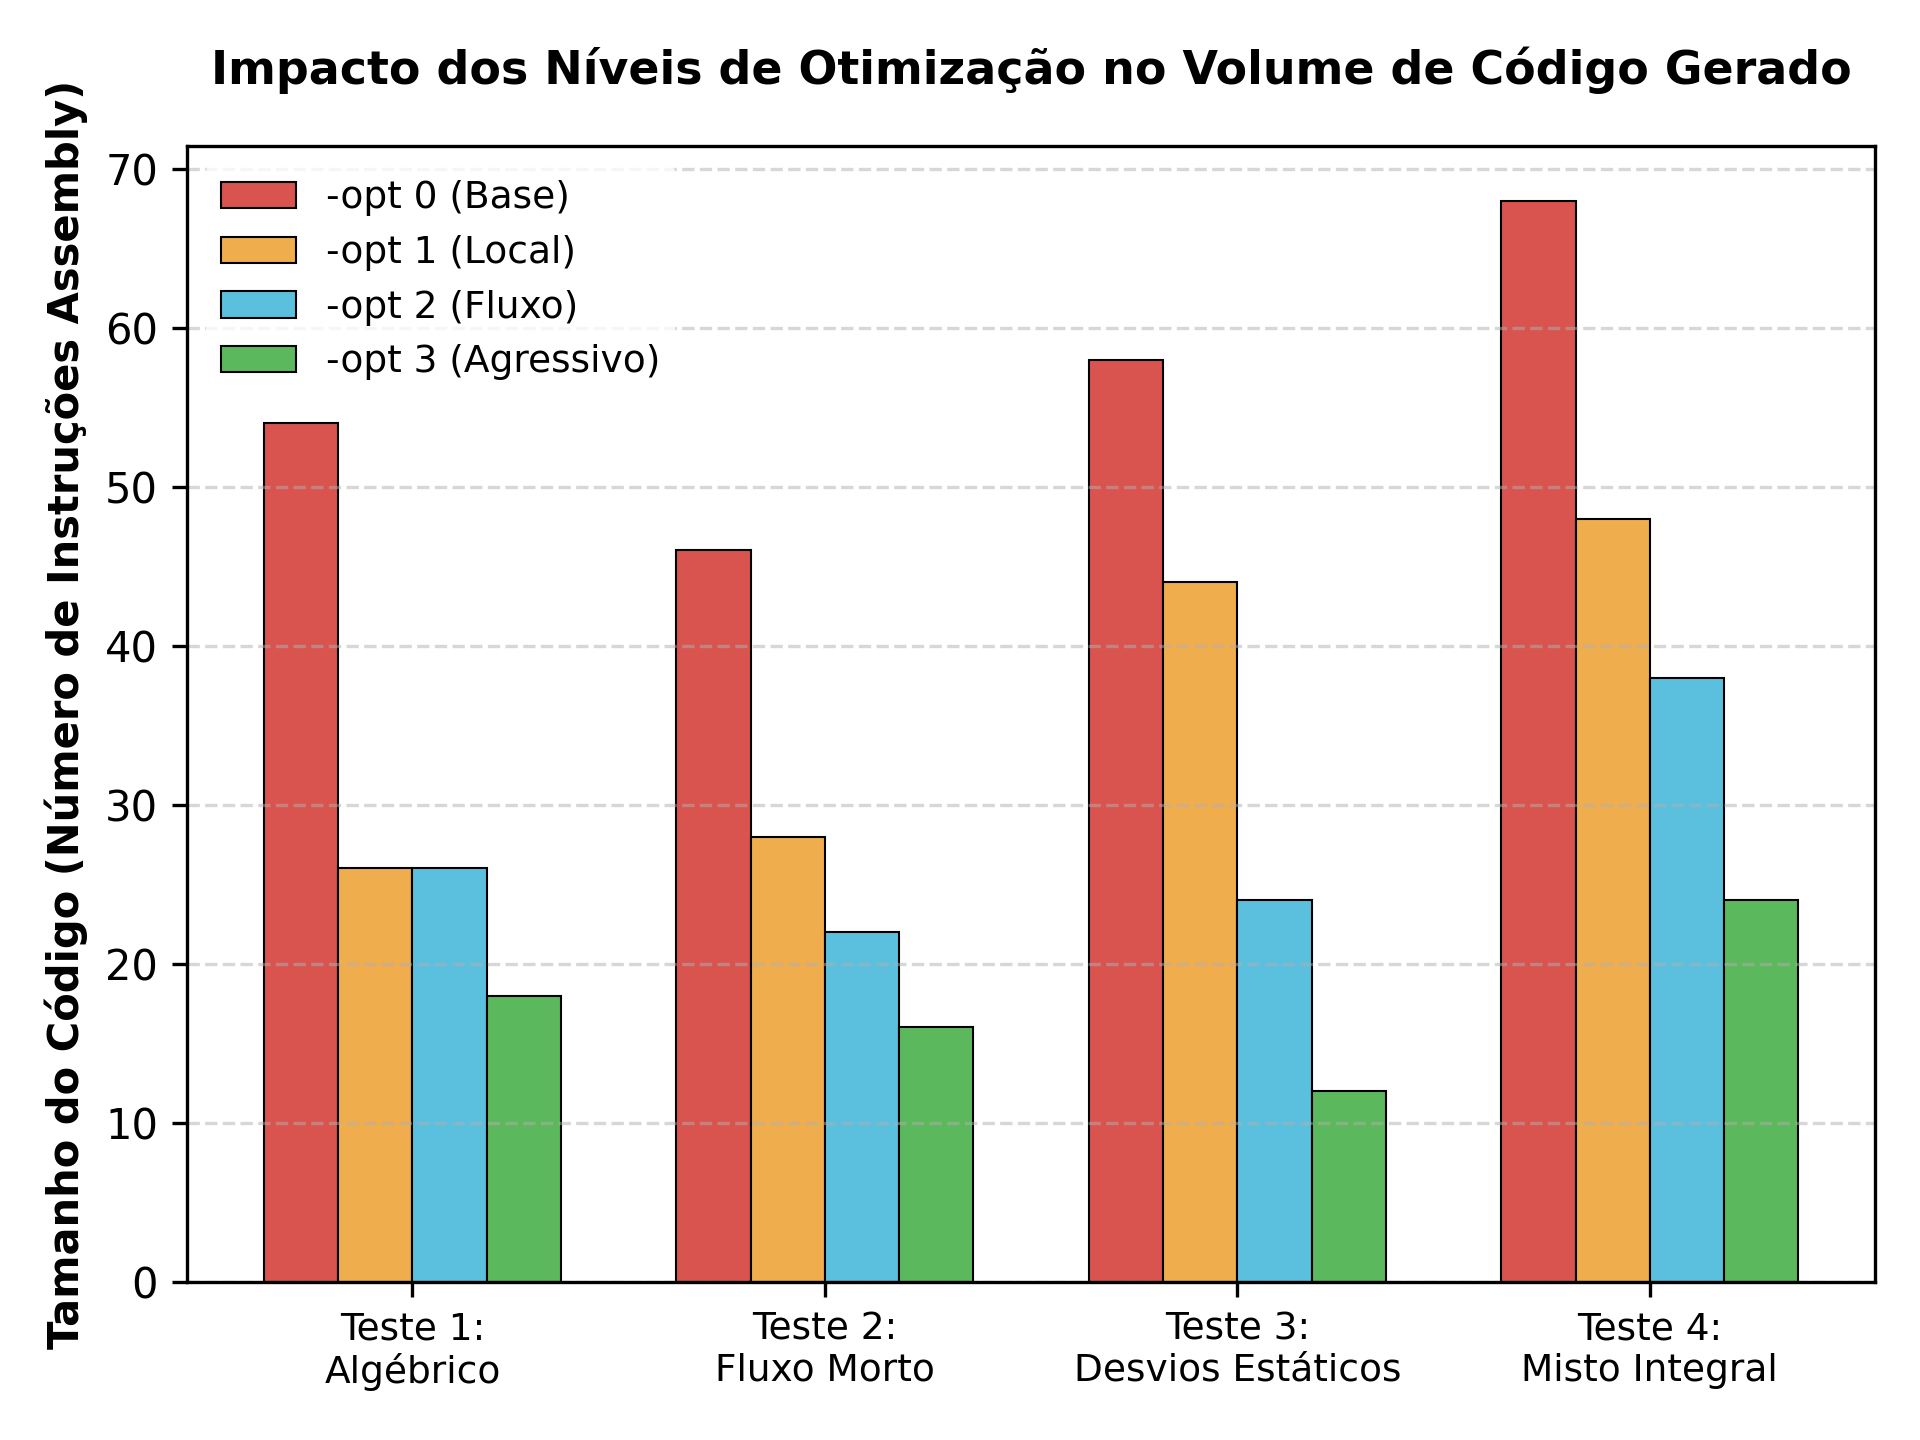
\includegraphics[width=0.85\textwidth]{evolucao_otimizacoes.png}
    \caption{Impacto dos níveis de otimização no volume de código gerado.}
    \label{fig:evolucao_otimizacoes}
\end{figure}

O comportamento dos testes face aos diferentes níveis de otimização, ilustrado na Figura~\ref{fig:evolucao_otimizacoes}, valida a arquitetura modular e incremental do sistema desenvolvido.

O teste \texttt{built\_ins} demonstra um cenário estável: mantém-se invariável entre o nível \texttt{-opt 0} e \texttt{-opt 1} (74 instruções) devido à ausência de constantes puras elegíveis para dobragem. Contudo, o nível \texttt{-opt 2} consegue reduzir o código para 66 instruções. Este ganho deve-se à eliminação de rótulos mortos e saltos redundantes que tinham sido gerados de forma automática pelas rotinas de conversão e pelo cálculo do valor absoluto (\texttt{\_emit\_abs}). O ponto fixo é consolidado no nível \texttt{-opt 3} com 64 instruções, onde o pipeline cíclico remove as redundâncias remanescentes.

Por outro lado, os testes \texttt{algorythm} e \texttt{flow} evidenciam uma flutuação nominal previsível: o volume de instruções no nível \texttt{-opt 2} (81 e 43 linhas, respetivamente) apresenta-se superior ao registado no nível \texttt{-opt 1} (71 e 27 linhas). Este fenómeno justifica-se pelo facto de o nível \texttt{-opt 2} isolar estritamente as otimizações de fluxo de controlo, omitindo por completo a dobragem algébrica de constantes aplicada no nível anterior. Em algoritmos com elevada densidade matemática, o ganho cumulativo de ambas as frentes de otimização só se manifesta na sua totalidade ao atingir o nível máximo de otimização agressiva (\texttt{-opt 3}), fixando os patamares mínimos absolutos de 71 e 20 instruções, respetivamente.


% --- Secção 3: Gramática ---
\section{Gramática Utilizada}
Abaixo apresenta-se a gramática BNF simplificada suportada pelo compilador:

\begin{lstlisting}[caption=Gramática BNF do Compilador]
program         ::= PROGRAM ID declarations_opt statements END function_defs_opt

function_defs_opt ::= function_def { function_def | subroutine_def }
                    | <vazio>

(* Declaracoes *)
declarations_opt ::= { declaration }
                   | <vazio>

declaration     ::= type declarator_list

type            ::= INTEGER | REAL | LOGICAL

declarator_list ::= declarator { COMMA declarator }

declarator      ::= ID
                  | ID LPAREN NUMBER RPAREN

(* Instrucoes *)
statements      ::= statement { statement }

statement       ::= assignment
                  | print_stmt
                  | read_stmt
                  | call_stmt
                  | if_stmt
                  | do_stmt
                  | goto_stmt
                  | label_stmt
                  | continue_stmt
                  | return_stmt

assignment      ::= varref EQUALS expression

print_stmt      ::= PRINT TIMES COMMA expression_list

read_stmt       ::= READ TIMES COMMA varref_list

varref_list     ::= varref { COMMA varref }

varref          ::= ID
                  | ID LPAREN expression_list RPAREN

call_stmt       ::= CALL ID LPAREN [ expression_list ] RPAREN

goto_stmt       ::= GOTO NUMBER

label_stmt      ::= NUMBER statement

continue_stmt   ::= CONTINUE

return_stmt     ::= RETURN

(* Estruturas de Controlo *)
if_stmt         ::= IF LPAREN expression RPAREN THEN
                        statements
                    [ ELSE statements ]
                    ENDIF | END

do_stmt         ::= DO NUMBER ID EQUALS expression COMMA expression
                  | DO NUMBER ID EQUALS expression COMMA expression COMMA expression

(* Subprogramas *)
function_def    ::= type FUNCTION ID LPAREN param_list RPAREN
                        declarations_opt
                        statements
                    END

subroutine_def  ::= SUBROUTINE ID LPAREN param_list RPAREN
                        declarations_opt
                        statements
                    END

param_list      ::= declarator_list | <vazio>

(* Expressoes *)
expression_list ::= expression { COMMA expression }

expression      ::= expression OP expression
                  | MINUS expression
                  | NOT expression
                  | LPAREN expression RPAREN
                  | ID
                  | ID LPAREN expression_list RPAREN
                  | literal

OP              ::= + | - | * | / | **
                  | .EQ. | .NE. | .LT. | .LE. | .GT. | .GE.
                  | .AND. | .OR.

literal         ::= NUMBER | STRING | .TRUE. | .FALSE.
\end{lstlisting}
\section{Testes}
Para testar o programa, utilizaram-se os testes fornecidos pela equipa docente, dos quais não obtivemos o output correto no conversor. Apesar da equipa ter tentado, não se conseguiu chegar a uma correção do \textit{output}, porém acreditamos, que se tivéssemos feito uma melhor gestão do tempo, teríamos sucedido. 
Além dos testes fornecidos, foram sendo adicionados testes complementares de modo a testar certos recursos que achamos serem necessários.

\section{Fluxo de Execução do Compilador}
O processo de compilação segue um modelo de \textit{pipeline} sequencial, onde cada fase transforma o programa fonte numa representação progressivamente mais próxima da linguagem da Máquina Virtual. O fluxo de dados e a interação entre os módulos desenvolvidos estão sistematizados na Figura~\ref{fig:compiler_flowchart}.

\begin{figure}[htbp]
\centering
\begin{tikzpicture}[
    node distance=1.6cm,
    every node/.style={fill=white, font=\small},
    block/.style={draw, rectangle, minimum width=3.5cm, minimum height=0.8cm, rounded corners=2pt, align=center, line width=0.6pt},
    data/.style={draw, rectangle, dashed, minimum width=3.5cm, minimum height=0.6cm, align=center, fill=gray!5, line width=0.5pt},
    arrow/.style={-latex, line width=0.6pt},
    support/.style={draw=blue!30, rectangle, minimum width=3.8cm, minimum height=0.8cm, rounded corners=2pt, align=center, fill=blue!5, line width=0.6pt}
]

    % Nós do Fluxo Principal
    \node (src) [data] {Código Fonte\\(\texttt{.f} / \texttt{.f77})};
    \node (lexer) [block, below of=src] {Análise Léxica\\(\texttt{lexer.py})};
    \node (tokens) [data, below of=lexer] {Sequência de \textit{Tokens}};
    \node (parser) [block, below of=tokens] {Análise Sintática\\(\texttt{parser.py})};
    \node (ast) [data, below of=parser] {Árvore Sintática\\Abstrata (AST)};
    \node (semantic) [block, below of=ast] {Análise Semântica\\(\texttt{semantic.py})};
    \node (ast_val) [data, below of=semantic] {AST Validada};
    
    % Fase: Otimizador de Alto Nível (AST)
    \node (astopt) [block, below of=ast_val] {Otimização da AST\\(\texttt{ast\_optimizer.py})};
    \node (ast_opt_data) [data, below of=astopt] {AST Otimizada};
    
    \node (codegen) [block, below of=ast_opt_data] {Geração de Código\\(\texttt{bm\_codegen.py})};
    \node (asm_raw) [data, below of=codegen] {Assembly Original};
    \node (optimizer) [block, below of=asm_raw] {Otimizador de Bytecode\\(\texttt{optimizer.py})};
    \node (asm_opt) [data, below of=optimizer] {Assembly Otimizado\\(\texttt{.asm})};

    % Nós Laterais (Tabelas de Suporte com estilo e espaçamento corrigidos)
    \node (symtab) [support, right of=semantic, xshift=4.3cm] {Tabela de Símbolos \\ \& Funções};
    \node (builtins) [support, right of=codegen, xshift=4.3cm] {Definições Intrínsecas\\(\texttt{builtin\_defs.py})};

    % Setas do Fluxo Principal
    \draw [arrow] (src) -- (lexer);
    \draw [arrow] (lexer) -- (tokens);
    \draw [arrow] (tokens) -- (parser);
    \draw [arrow] (parser) -- (ast);
    \draw [arrow] (ast) -- (semantic);
    \draw [arrow] (semantic) -- (ast_val);
    \draw [arrow] (ast_val) -- (astopt);
    \draw [arrow] (astopt) -- (ast_opt_data);
    \draw [arrow] (ast_opt_data) -- (codegen);
    \draw [arrow] (codegen) -- (asm_raw);
    \draw [arrow] (asm_raw) -- (optimizer);
    \draw [arrow] (optimizer) -- (asm_opt);

    % Setas de Interação Lateral (Alinhamento milimétrico pelo corredor central)
    \draw [arrow, <->] (semantic) -- (symtab);
    \draw [arrow, ->] (symtab.south) -- ++(-2.3,0) |- ([yshift=0.15cm]codegen.east);
    \draw [arrow, ->] (builtins.west) -- ([yshift=-0.15cm]codegen.east);

    % Setas de Bypass Opcional (Lado Esquerdo)
    \draw [arrow, dashed] (ast_val.west) -- ++(-1.5,0) |- node[left, pos=0.25, align=center, font=\footnotesize] {Sem\\otimização} (codegen.west);
    \draw [arrow, dashed] (asm_raw.west) -- ++(-1.5,0) |- node[left, pos=0.25, align=center, font=\footnotesize] {Sem\\otimização} (asm_opt.west);

\end{tikzpicture}
\caption{Fluxo de dados e arquitetura modular do compilador com dupla fase de otimização opcional.}
\label{fig:compiler_flowchart}
\end{figure}

\newpage
\section{Compilação e Utilização}
Para compilar um ficheiro Fortran utilizando a interface de linha de comandos desenvolvida, utilize o seguinte formato de comando no terminal:
\begin{lstlisting}[language=bash]
python src/__main__.py main <ficheiro.f> <nivel_opt> <saida.asm>
\end{lstlisting}

Onde \texttt{<nivel\_opt>} corresponde a um valor numérico inteiro de 0 a 3.

% --- Secção 7: Dificuldades ---
\section{Dificuldades de Implementação}

Durante o desenvolvimento do compilador, o grupo enfrentou alguns desafios técnicos complexos relacionados com as restrições físicas e estruturais da Máquina Virtual (VM) de destino:

\begin{enumerate}
    \item Ambiguidade entre acesso a array e chamada de função: Em Fortran, A(5) pode ser tanto aceder ao índice 5 de um array como chamar uma função chamada A. O parser não consegue distinguir os dois casos só pela sintaxe, por isso trata ambos como chamada de função. A distinção só é feita mais tarde, no gerador de código, consultando a tabela de símbolos.
    \item Estrutura dos ciclos DO: O Fortran não delimita os ciclos DO com chavetas nem palavras-chave de fecho — o ciclo termina quando aparece um número de linha específico noutro sítio do código. Isto significa que o parser gera o DoStmt sem body, e foi necessário implementar uma rotina no analisador semântico que percorre a lista de instruções e move as que pertencem ao ciclo para dentro do nó correcto.
    \item O END fecha múltiplas coisas: A palavra END é usada para terminar o programa principal, funções, subrotinas, e também pode terminar um IF. Isto causou conflitos no parser que tiveram de ser resolvidos com regras específicas — por exemplo, criando uma regra endif que aceita tanto ENDIF como END.
    
\end{enumerate}

\section{Conclusão}
O desenvolvimento deste projeto permitiu consolidar na vertente prática os conceitos fundamentais de engenharia de linguagens, traduzidos na implementação bem-sucedida de um pipeline completo de compilação para um subset expressivo da linguagem Fortran 77. 

A resolução de problemas clássicos, tais como o desdobramento e normalização de laços de controlo não delimitados e o tratamento de assinaturas de chamadas ambíguas entre vetores e funções, forneceu um entendimento aprofundado acerca da abstração fornecida por linguagens de alto nível. Por fim, o desenvolvimento do sistema integrado de dupla fase de otimização provou o impacto direto da análise estática de código na economia de recursos de memória e na eficiência de processamento no ambiente da Máquina Virtual de destino.

\end{document}